%%%%%%%%%%%%%%%%%%%%%%% file template.tex %%%%%%%%%%%%%%%%%%%%%%%%%
%
% This is a general template file for the LaTeX package SVJour3
% for Springer journals.          Springer Heidelberg 2010/09/16
%
% Copy it to a new file with a new name and use it as the basis
% for your article. Delete % signs as needed.
%
% This template includes a few options for different layouts and
% content for various journals. Please consult a previous issue of
% your journal as needed.
%
%%%%%%%%%%%%%%%%%%%%%%%%%%%%%%%%%%%%%%%%%%%%%%%%%%%%%%%%%%%%%%%%%%%
%
% First comes an example EPS file -- just ignore it and
% proceed on the \documentclass line
% your LaTeX will extract the file if required
\begin{filecontents*}{example.eps}
%!PS-Adobe-3.0 EPSF-3.0
%%BoundingBox: 19 19 221 221
%%CreationDate: Mon Sep 29 1997
%%Creator: programmed by hand (JK)
%%EndComments
gsave
newpath
  20 20 moveto
  20 220 lineto
  220 220 lineto
  220 20 lineto
closepath
2 setlinewidth
gsave
  .4 setgray fill
grestore
stroke
grestore
\end{filecontents*}
%
\RequirePackage{fix-cm}
%
%\documentclass{svjour3}                     % onecolumn (standard format)
%\documentclass[smallcondensed]{svjour3}     % onecolumn (ditto)
\documentclass[smallextended]{svjour3}       % onecolumn (second format)
%\documentclass[twocolumn]{svjour3}          % twocolumn
%
\smartqed  % flush right qed marks, e.g. at end of proof
%
\usepackage{graphicx}
\usepackage{natbib}
%
% \usepackage{mathptmx}      % use Times fonts if available on your TeX system
%
% insert here the call for the packages your document requires
%\usepackage{latexsym}
% etc.
%
% please place your own definitions here and don't use \def but
% \newcommand{}{}
%
% Insert the name of "your journal" with
 \journalname{Climate Dynamics}
%
\begin{document}

\title{Heatwaves for EuroCORDEX future climate simulations
%\thanks{Grants or other notes
%about the article that should go on the front page should be
%placed here. General acknowledgments should be placed at the end of the article.}
}
\subtitle{Do you have a subtitle?\\ If so, write it here}

%\titlerunning{Short form of title}        % if too long for running head

\author{M. O. Molina         \and
        E. Sánchez %etc.
}

%\authorrunning{Short form of author list} % if too long for running head

\institute{Faculty of Environmental Sciences and Biochemistry. University of Castilla-La Mancha 
\at Avenida Carlos III s/n, 45071-Toledo  \\
              \email{MOfelia.Molina1@alu.uclm.es}           %  \\
%             \emph{Present address:} of F. Author  %  if needed
           \and
           S. Author \at
              second address
} 
 
\date{Received: date / Accepted: date}
% The correct dates will be entered by the editor


\maketitle

\begin{abstract}
Insert your abstract here. Include keywords, PACS and mathematical
subject classification numbers as needed.
\keywords{First keyword \and Second keyword \and More}
% \PACS{PACS code1 \and PACS code2 \and more}
% \subclass{MSC code1 \and MSC code2 \and more}
\end{abstract}

\section{Introduction}
\label{introduction}
The main paper about eurocordex is \cite{jac_al2014}. Present climate
modelling of heatwaves was described by \cite{vau_al2013}.

Present climate modelling of heat waves at the regional scale of Europe was described by \cite{vau_al2013}, so in this paper the evolution of the heat waves under climate change effects in the future period over Europe is evaluated.

A heat wave is defined as a period of consecutive days with hot temperatures. There is a type of heat wave, more extreme still, called "mega heat waves". The two hottest events have occured in the last decade \cite{bar_al2011} with importants effects on society. 

Synoptic sistems that produce heat waves are high prresures and dry soil moisture. From a metheorogical point of view, a heat wave event is produce when a stationary high pressure sistem remains in the same location for a longer period than expected. The high pressure system cause and prolong a heat wave event by advecting warm dry air to the region afected. On the other hand, extreme temperatures are more likely when soil moisture decreases. Dry moistures wuth persistent high pressures conditions amplifies the positive feedback \cite{per2015}. A clear spatial correlation between antecedent soil moisture conditions and heat wave temperatures was shown by \cite{Sil_al2017} for the European heat waves of 2003 and 2010. 
 

The Expert Team on Climate Change Detection and Indices (ETCCDI) has defined several indices to measure extreme temperatures. They are derived from daily maximum and minimum temperature and daily precipitation.    

\section{Data: Simulations and models}

Temperature extremes require high-quality daily data for their calculation \cite{per2015}. The data have been provided by EURO-CORDEX, the European branch of the CORDEX initiative. The EURO-CORDEX simulations are based on multiple dynamical and empirical-statistical downscaling models forced by multiple global climate models from the Coupled Model Intercomparison Project Phase 5 (CMIP5). Daily maximum temperatures of historical simulations are used for period () and are compared with simulations for future periord (). Future climate simulations are based on greenhouse gas emission scenarios (Representative Concentration Pathways, RCPs) corresponding to stabilization of radiative forcing after the 21st century at 4,5 W/m² (RCP4.5) and a rising radiative forcing crossing 8,5 W/m² at the end of 21st century (RCP8.5) \cite{Mos_al2010}. 
A comparison of several simulations couples are analyzed in detail to improve our understanding of the uncertainities related to heat wave description: two RCMs forced with the same GCM, two different emissions scenarios for the same RCM, and the effect of resolution 0.44 vs 0.11. 


\section{Methods}

In this study we use two indices to asses projected changes in the intensity and duration of the heat waves over Europe. Almost every climatological study about heat waves  uses a different metric, so we have selectionate one index to asses the frecuency and another one to study the intensity of the heat waves  in the future. The election of the correct index depends on the objetive of the study. Extreme temperature indices are based in thresholds of temperature that can vary if you are studying its effects of temperature on health or in agriculture.  In climate, this threshold can not be a fixed temperature because the daily temperature variability is different among regions.  So that, the ETCCDI replaced the HWDI index (Frich et al., 2002) by the Spell Warm Duration Index (SWDI), which is calculated using a percentile-based threshold.     

The Heat Wave Magnitude Index is defined as the maximum magnitude of the heat waves in a year, where heat wave is the period ≥ 3 consecutive days with maximum temperature above the daily threshold for the reference period 1981–2010. The threshold is defined as the 90th percentile of daily maxima, centered on a 31 day window \cite{rus_al2014}.

The Warm Spell Duration Index (WSDI) is defined as follows: Let TX ij be the daily maximum temperature on day i in period j and let TX in 90 be the calendar day 90 th percentile centered on a 5 day window for the base period 1961–1990. Then the number of days per period is summed where, in intervals of at least 6 consecutive days: TX ij > TX in 90.

The calculations are performed with the R package climdex.pcic as documented at The Comprehensive R Archive Network website (http://cran.r-project.org/web/packages/climdex.pcic/index.html).  

Kike (pruebas): The main index we will use is HWDI \citep{rus_al2014}


As shown in section \ref{intro}
\label{sec:1}
%Text with citations \cite{RefB} and \cite{RefJ}.
\subsection{Subsection title}
\label{sec:2}
as required. Don't forget to give each section
and subsection a unique label (see Sect.~\ref{sec:1}).
\paragraph{Paragraph headings} Use paragraph headings as needed.
\begin{equation}
a^2+b^2=c^2
\end{equation}

% For one-column wide figures use
\begin{figure}
% Use the relevant command to insert your figure file.
% For example, with the graphicx package use
  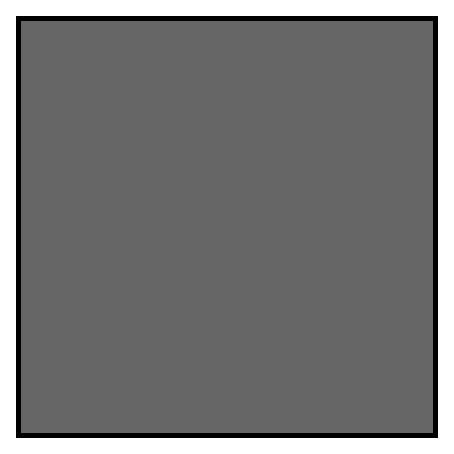
\includegraphics{example.eps}
% figure caption is below the figure
\caption{Please write your figure caption here}
\label{fig:1}       % Give a unique label
\end{figure}
%
% For two-column wide figures use
\begin{figure*}
% Use the relevant command to insert your figure file.
% For example, with the graphicx package use
  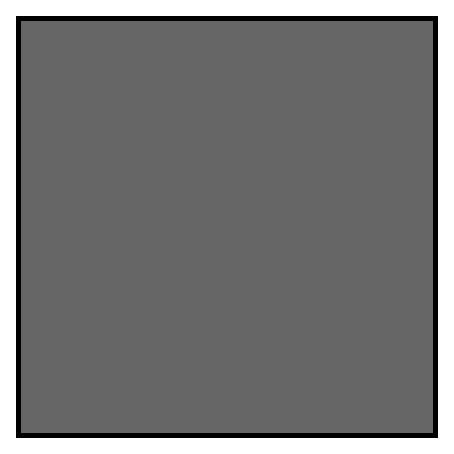
\includegraphics[width=0.75\textwidth]{example.eps}
% figure caption is below the figure
\caption{Please write your figure caption here}
\label{fig:2}       % Give a unique label
\end{figure*}
%
% For tables use
\begin{table}
% table caption is above the table
\caption{Please write your table caption here}
\label{tab:1}       % Give a unique label
% For LaTeX tables use
\begin{tabular}{lll}
\hline\noalign{\smallskip}
first & second & third  \\
\noalign{\smallskip}\hline\noalign{\smallskip}
number & number & number \\
number & number & number \\
\noalign{\smallskip}\hline
\end{tabular}
\end{table}


%\begin{acknowledgements}
%If you'd like to thank anyone, place your comments here
%and remove the percent signs.
%\end{acknowledgements}

% BibTeX users please use one of
\bibliographystyle{spbasic}      % basic style, author-year citations
%\bibliographystyle{spmpsci}      % mathematics and physical sciences
%\bibliographystyle{natbib}
%\bibliographystyle{spphys}       % APS-like style for physics
\bibliography{climabibtotal}   % name your BibTeX data base

% Non-BibTeX users please use
%\begin{thebibliography}{}
%
% and use \bibitem to create references. Consult the Instructions
% for authors for reference list style.
%
%\bibitem{RefJ}
% Format for Journal Reference
%Author, Article title, Journal, Volume, page numbers (year)
% Format for books
%\bibitem{RefB}
%Author, Book title, page numbers. Publisher, place (year)
% etc
%\end{thebibliography}

\end{document}
% end of file template.tex

